\section{Background: A Brief Tour of CompCert}
\label{sec:background}

We begin by briefly reviewing the technical background that informs the rest of this dissertation,
using CompCert as the learning material.  The technical ideas and results presented in this section
apply not only to CompCert but also to other compilers as well.  We first explain CompCert's
correctness statement, as well as its simulation verification technique
(\Cref{sec:background:correctness}).  To flesh out the details on formal semantics and compiler
verification, we use RTL---one of CompCert's internal representations---and constant
propagation---one of CompCert's optimizations---as a running example.  Specifically, We first review
CompCert's memory model that is specifically designed so as to verify compiler optimizations
(\Cref{sec:background:memory}).  Then we explain the RTL language on which constant propagation and
most of the other optimizations are performed in the CompCert's compilation pipeline
(\Cref{sec:background:rtl}), and how constant propagation works and how CompCert verifies it
(\Cref{sec:background:constprop}).  Throughout this section, we keep the presentation semi-formal,
abstracting away unnecessary detail to get across the main ideas.  For more details, we refer the
reader to \cite{compcert, compcert-memory-model}.


\subsection{Compiler Correctness}
\label{sec:background:correctness}

\paragraph{End-to-End Correctness}

Roughly speaking, the correctness result of CompCert can be understood to assert \emph{semantic
  preservation}, which in turn means the following.  Suppose \code{s.c} is a ``source'' file (in C),
\code{t.asm} is a ``target'' file (in assembly), and $\mathcal{C}$ is a verified compiler
(represented as a function from C files to assembly files).
\[
\frac{
\mathcal{C}(\mathtt{s.c}) = \mathtt{t.asm} \qquad
s = \mathrm{load}(\mathtt{s.c})\qquad
t = \mathrm{load}(\mathtt{t.asm})}
{\mathrm{Behav}(s) \supseteq \mathrm{Behav}(t)}
\]
If \code{t.asm} is the result of compiling \code{s.c} with $\mathcal{C}$, then executing
\code{t.asm} according to assembly semantics will result in a subset of the behaviors one could
observe from executing \code{s.c} according to C semantics.  (We write
$s = \mathrm{load}(\mathtt{s.c})$ to denote the \emph{machine state} that results from loading
$\mathtt{s.c}$ into memory, $\mathrm{Behav}(s)$ to denote the observable behaviors of the execution
of $s$, and analogously for $t$ and $\mathtt{t.asm}$.)  Hence, we say that \code{t.asm}, the
target-level output of $\mathcal{C}$, \emph{refines} its source-level input, \code{s.c}.

The compiler correctness statement presented here will be generalized to support separate
compilation in \Cref{chap:sepcomp}.


\paragraph{Set of Behaviors}

% The standard notion of compiler correctness is behavioral refinement, which states that \emph{the
%   set of target program behaviors must be a subset of the set of source program behaviors}.
We consider sets of behaviors as opposed to single behaviors because a program may produce multiple
behaviors due to nondeterminism.  Given a set of I/O events that programs may generate and users may
observe, a behavior is one of the following three forms: $(1)$ a terminating execution producing a
finite sequence of I/O events, $e_1, \cdots, e_n, \mathtt{term}$; $(2)$ a diverging execution that
has produced only a finite sequence of I/O events, $e_1, \cdots, e_n, \mathtt{nonterm}$; and $(3)$ a
diverging execution producing an infinite sequence of I/O events, $e_1, \cdots, e_n, \cdots$.

Undefined behavior requires special attention in defining the set of behaviors, because the program
states in the condition are neither terminated nor transitioning to other states, fitting into none
of the behavioral categories.  We assign \emph{the set of all behaviors} to the program states
invoking undefined behavior in order to validate compiler optimizations: if the source program's
behavior is undefined, then compiler can choose any program as its result; on the other hand, if the
target program's behavior is undefined, then the source program's behavior should also be undefined.
% We regard \emph{the undefined behavior as described in the ISO C standards as the set of all
% behaviors}.  This captures the intuitive properties of compilers on undefined behavior.


\paragraph{Per-Pass Correctness}

To verify compilation correctness for the compiler $\mathcal{C}$, CompCert verifies each pass of
$\mathcal{C}$ independently.  Specifically, for each pass (transformation) $\mathcal{T}$ from
language $L_1$ to $L_2$---where the $L_i$'s may be C, assembly, or some intermediate languages---we
show the following:
\[
\frac{
\mathcal{T}(\mathtt{s.l1}) = \mathtt{t.l2} \qquad
s = \mathrm{load}(\mathtt{s.l1}) \qquad
t = \mathrm{load}(\mathtt{t.l2})
}
{
\mathrm{Behav}(s) \supseteq \mathrm{Behav}(t)
}
\]
That is, given the input \code{s.l1} and output \code{t.l2} of the $\mathcal{T}$ transformation, we
show that the behaviors of \code{t.l2} are contained within those of \code{s.l1}.  Since subset
inclusion is transitive, it easy to see that the proofs of the constituent passes of $\mathcal{C}$
compose to establish the correctness of $\mathcal{C}$ as a whole.

% \begin{figure}[!t]
% \begin{center}
% 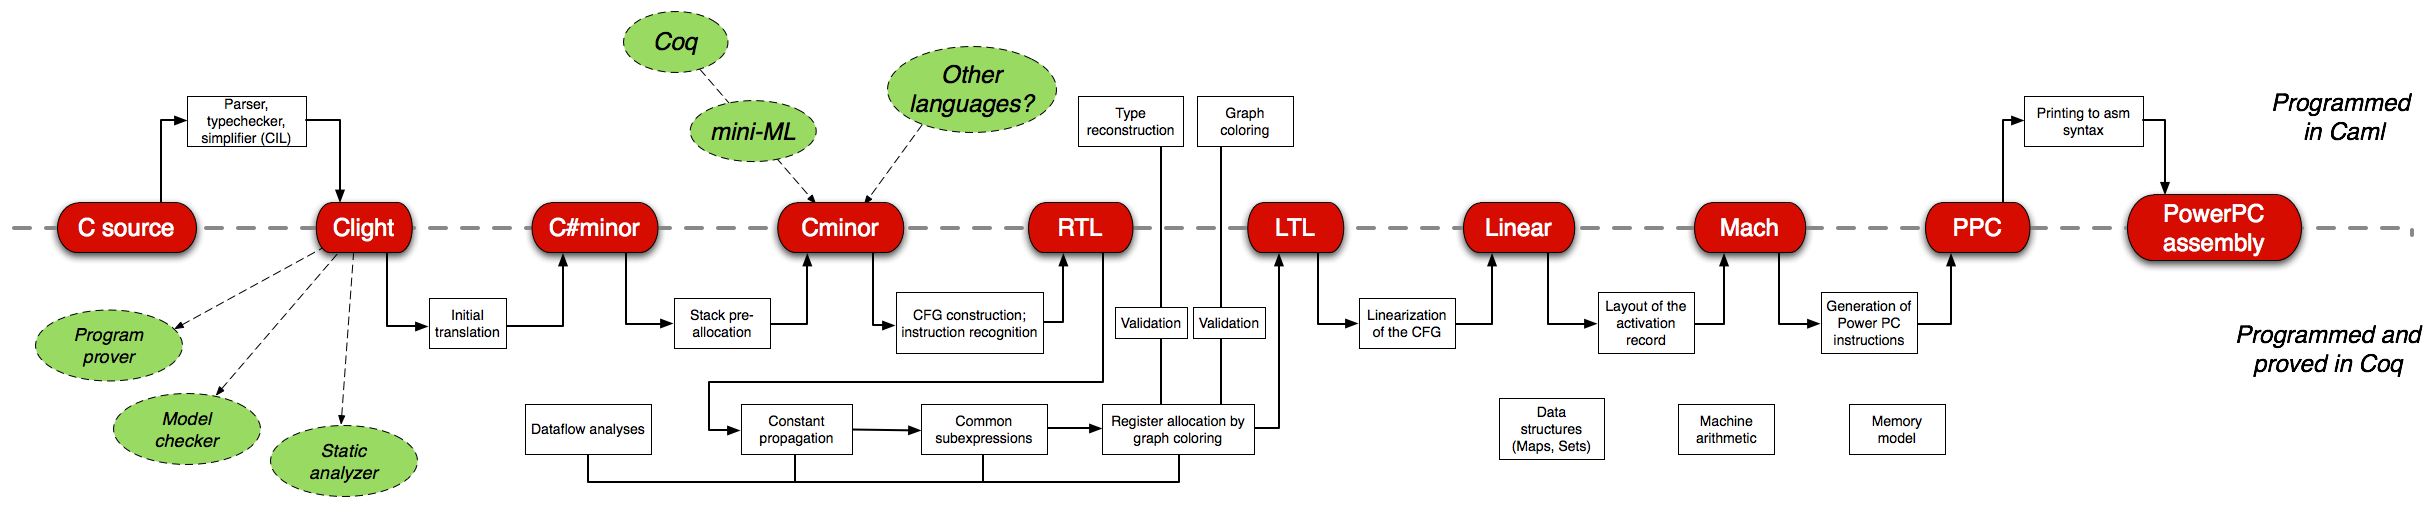
\includegraphics[width=\textwidth]{compcert-diagram.png}
% \end{center}
% \caption{Organization of CompCert (from~\cite{compcert-web})  \jeehoon{too old, change it}}
% \label{fig:compcert-organization}
% \end{figure}

% It is worth noting that CompCert consists of \jeehoon{10} optimization and transformation passes
% that go through \jeehoon{10} intermediate languages, as illustrated in
% \Cref{fig:compcert-organization}.  On the other hand, Mainstream compilers typically have dozens of
% passes.


\paragraph{Verifying Per-Pass Correctness}

Now how does one actually prove the verification condition for each individual pass?  The standard
approach taken by CompCert is to use (closed) simulations.  Informally, we will say that a
\emph{simulation} $R$ is a relation between running programs (\ie machine states) in $L_1$ and $L_2$
such that, if $(s,t) \in R$, then the behaviors one observes while stepping through the execution of
$t$ are matched by corresponding observable behaviors in the execution of $s$.  One can think of $R$
as imposing an invariant, which describes (and connects) the possible machine states of the source
and target programs, and which must be maintained as the programs execute.  We leave further details
about simulations until \Cref{sec:background:constprop}; suffice it to say that they satisfy the
following ``adequacy'' property:
% , and we show that the machine states arising from
% loading \code{s.l1} and \code{t.l2} belong to this simulation.
\[
\frac{
R~\mbox{is a simulation} \qquad
(s,t)\in R
}{
\mathrm{Behav}(s) \supseteq \mathrm{Behav}(t)
}
\]
Thus, to establish the verification condition for pass $\mathcal{T}$, it suffices to exhibit a
simulation $R$ that relates $\mathrm{load}(\mathtt{s.l1})$ and $\mathrm{load}(\mathtt{t.l2})$.



\paragraph*{}

In the rest of this section, we flesh out the details on formal semantics and compiler verification
in CompCert, using constant propagation as the running example.  Constant propagation is essentially
a transformation that optimizes memory operations, so we will first review their semantics in
CompCert.

% At the essence of the compiler optimization is memory operations, so we will first review their
% semantics in CompCert.


\subsection{Memory Model}
\label{sec:background:memory}


CompCert supports the following memory operations:
\[
\begin{array}{r@{~~}c@{~~}l}
  \memLoad &\in& \rtlMem \to \rtlAddr \to \powset{\rtlVal} \\
  \memStore &\in& \rtlMem \to \rtlAddr \to \rtlVal \to \powset{\rtlMem} \\
  \memMalloc &\in& \rtlMem \to \usize \to \powset{\rtlAddr \times \rtlMem} \\
  \memFree &\in& \rtlMem \to \rtlAddr \to \powset{\rtlMem} \\
\end{array}
\]
%
\noindent Memory, $m\in\rtlMem$, supports four operations: load, store, malloc, and free.  Note that
all operations may produce multiple results due to the nondeterminism arising from \eg{}
concurrency.  A load operation reads the value, $v\in\rtlVal$, of an address, $a\in\rtlAddr$, and a
store operation writes a value to an address in the memory.  If a load or store operation access an
illegal address, then there are no valid results.  A malloc operation allocates a memory object of
the specified size of type $\usize$ (the set of 32-bit unsigned integers), returning the new memory
and the address of the allocated object, and a free operation deallocates an allocated memory
object.

Now we define the semantic domain for and the semantics of those memory operations, or in other
words, define the \emph{memory model}.  The memory model presented here will be generalized to
support integer-pointer casts and relaxed-memory concurrency in \Cref{chap:intptrcast} and
\Cref{chap:relaxed}, respectively.

To simplify the presentation, we do not discuss many aspects of C memory models that are orthogonal
to the contributions of this dissertation.  Specifically, we $(1)$ assume a 32-bit architecture:
words are 4 bytes wide and the size of the address space is $2^{32}$, as eminent from the signature
of $\memMalloc$; $(2)$ consider only unsigned integer and pointer values, and omit values of other
types such as \isize, \code{float} or \code{char}; and $(3)$ omit subword arithmetic, and assume
each address stores a 32-bit value.

% and take all addressing to be aligned at 4-byte boundaries.  \todo{gil: this is not quite
% right. For example, we have a 4-byte word at 0x0000FFF0 and another 4-byte word at 0x0000FFF1,
% ratherthan at 0x0000FFF4.  We used this just for simplicity anyway.}  $(l,i)$ points to the $i$-th
% cell of 4 byte data in the logical block $l$).

% Roughly speaking, a memory model defines which value(s) a load operation can read from



\paragraph{Concrete Model}

The most straightforward way to define a memory model is closely following the hardware assembly
language: pointers have the same representation as integer values of the appropriate width, and they
simply index into a single flat array representing memory.  In such a \emph{concrete memory model},
memory consists of a $2^{32}$-sized array of values, and a list of allocated blocks, represented as
pairs $(p,n)$ of the block's starting address and its size.  Loading from or storing to an
unallocated address raises an error (\ie undefined behavior).  Values are just 32-bit integers,
since pointers are merely integers in the concrete model.  As a result, \emph{the concrete model
  natively supports integer-pointer casts}.
\[
\begin{array}{@{}l@{~}c@{~}l@{}}
\mathrm{Mem} &\defeq& (\usize \to \rtlVal) \times \mathtt{list}\ \mathrm{Alloc} \\
\mathrm{Alloc} &\defeq& \setof{(p,n) \suchthat p \in \usize \land n \in \usize} \\
\rtlVal &\defeq& \setof{i\in\usize}
\end{array}
\]

Memory allocation inserts a block into the list of allocated blocks, whereas deallocation removes
one.  Overall, the list of allocated blocks should be \emph{consistent}:\footnote{These are a subset
  of \code{malloc}'s properties according to the C11 standard~\cite{iso2011iec}.  For more details,
  see \S7.22.3 paragraph~1 and \S6.5.8 paragraph~5. \jeehoon{Update to C18}}
\begin{itemize}
\item If $(p, n)$ is allocated, then $\emptyset \neq [p,p+n) \subseteq
  (0,2^{32}-1)$.
%\item If $(p, n)$ is allocated, then $p\neq 0$ and $n\neq 0$.
\item If blocks $(p_1, n_1)$ and $(p_2, n_2)$ are distinct
  allocations, their ranges $[p_1,p_1+n_1)$ and $[p_2,p_2+n_2)$
  are disjoint.
\end{itemize}

As we have seen in \Cref{sec:introduction:context}, however, the concrete model \emph{does not
  support standard compiler optimizations} such as constant propagation in the presence of external
function calls.  This is because the model does not provide a mechanism for ensuring that a module
has exclusive control over some part of memory, thereby assuming that unknown code can read and
update the contents of every allocated memory cell.

\jeehoon{The concrete model also invalidates dead allocation elimination optimizations.  Connect it
  to the logical memory model's advantages.}

\jeehoon{In the above example, the first optimization is allowed since there is no way to forge the
  logical address of the variable \code{a} from those of other blocks. Also, the second one is
  allowed since the memory is infinitely large.}

\jeehoon{where typically the set of valid allocation block identifiers is infinite.  While logical
  models allow most compiler optimizations, the problem is that}

\jeehoon{Connect logical model and C18.  What's C18, actually?}

Consider, for example, a function \code{f} that initializes a local variable \code{a} and then calls
some unknown external function~\code{g}. We might expect the compiler to deduce that the value of
\code{a} is unaffected by the call to \code{g} and perform constant propagation:
%% On the formal side, there are two types of memory models for C\@.
% On the one hand, we have \emph{concrete} models.
% These represent pointers as 32-bit (or 64-bit) integers,
% which is close to what programmers expect, but do not support
% some of even the most basic optimizations that compilers perform.
% As a simple illustration, consider the following function \code{f} that
% initializes a local variable \code{a} and then calls some unknown external
% function \code{g}.
% The compiler might perform constant propagation and optimize this program
% as follows by assuming that the value of \code{a} is unaffected by the call to \code{g}.
\begin{center}
\begin{tabular}{@{}l@{}l@{}l@{}l@{}l@{}}
%% \small
\begin{minipage}{0.2\textwidth}
\small
\begin{minted}{c}
extern void g();

int f(void) {
  int a = 0;
  g();
  return a;
}
\end{minted}
\end{minipage}
&
$\quad\rightarrow\quad$
&
%% \small
\begin{minipage}{0.2\textwidth}
\small
\begin{minted}{c}
extern void g();

int f(void) {
  int a = 0;
  g();
  return 0;
}
\end{minted}
\end{minipage}
&
$\quad\rightarrow\quad$
&
%% \small
\begin{minipage}{0.2\textwidth}
\small
\begin{minted}{c}
extern void g();

int f(void) {

  g();
  return 0;
}
\end{minted}
\end{minipage}
\\
\end{tabular}
\end{center}

\vskip 0.3cm Using a simple concrete memory model, however, we have to consider the possibility that
\code{g} is able to ``guess'' the location of \code{a} in memory and changes its value. This can
happen if, for instance, our semantics allocates memory deterministically and the caller
of~\code{f} sets up the state of memory appropriately for \code{g}.

% We note, however, that this reasoning is not valid in the concrete model.
% The variable \code{a} is allocated somewhere in memory, and the external
% function might `guess' the address at which it is allocated and overwrite
% its value.
%

The compiler may further optimize the program by completely removing
the now unused local variable \code{a}. This latter transformation is again
disallowed by concrete models because it might change the behavior of
the program:
by virtue of there being one fewer memory cells allocated, the call to \code{g}
might succeed where initially it exhausted memory.



\paragraph{CompCert's Logical Model}

In order to support standard compiler optimizations, CompCert is based on a \emph{logical} memory
model~\cite{leroy:compcert,Leroy-Appel-Blazy-Stewart-memory-v2} rather than the naive concrete
model.  In the logical model, memory is a finite collection of logical blocks with unique block
identifiers, together with the maximum of the allocated block identifiers.  Each block is a
contiguous, fixed-sized array of values annotated with a validity flag $v$ that indicates whether
the block is accessible or has been freed. As before, accessing a freed block raises an error.
Values are either 32-bit integers, logical addresses, or the special \emph{undefined value} that
represents uninitialized data.  Here, a logical address $(l,i)$ consists of a block identifier $l$
and an offset $i$ inside the block.
% (For simplicity, throughout this paper, we assume pointers
%are aligned at 4-byte boundaries and $(l,i)$ represents the 4-byte chunk at
%offset $4i$. \todo{This is not right for the same reason as before.})
%For a block identifier $l$, we henceforth write the 
%block $l$ for the block with identifier $l$.
\[
\begin{array}{@{}l@{~}c@{~}l@{}}
\rtlMem &\defeq& \setof{(nb,bs)\suchthat nb\in\rtlBId\land bs \in \rtlBId \fpfun \rtlBlock} \\
\rtlBlock &\defeq&
\setof{(v, n, c) \suchthat
  v \in \setofz{\rtlvalid,\rtlfreed} \land n \in \Nat \land c \in \rtlVal^n } \\
\rtlVal &\defeq& \setof{i\in\usize} \uplus \rtlAddr \uplus \setofz{\rtlundef} \\
\rtlAddr &\defeq& \setof{(l,i) \in \rtlBId\times \usize}
\end{array}
\]

An important advantage of the logical model over the concrete one is that 
it \emph{allows functions to have exclusive control over a logical block} as 
long as they do not allow its address to escape. The reason is that it
is not possible to manufacture the logical address of an already allocated block.  
This property guarantees the correctness of many useful optimizations, 
such as constant propagation across function calls and dead allocation
elimination.

A secondary advantage is that programs have \emph{infinite memory}, rendering
their allocation behavior unobservable, which in turn makes it easy for
compilers to remove dead allocations.

%% there is no out-of-meory behavior since the memory has infinitely many logical blocks.
%This is important because even if a source program consumes a huge
%amount of memory, ... (\todo{Viktor, please say something about this
% :)})

Apart from that logical models have a slightly more complicated semantics, their main disadvantage
is that \emph{they do not support integer-to-pointer casts} very well.  As a result, CompCert does
not support real-world use cases of integer-pointer casts well.
%% The main disadvantages of logical models are that they have a slightly more complicated semantics
%% and, most importantly, that \emph{they do not support integer-to-pointer casts} very well.
Specifically, they are treated as \code{nop}s (\ie the identity function), and thus variables of
integer (or pointer) types can contain both integers and logical addresses.  This conflicts with the
intention of integer-pointer casts to freely manipulated pointers as if they are integer values.  We
will address this disadvantage in \Cref{chap:intptrcast}.

% In CompCert's higher-level languages (CompCert C and Clight), once a pointer is cast into an
% integer, any arithmetic on that integer returns an unspecified value.  In its lower-level languages
% (Cminor, RTL, \emph{etc.}), however, some of the integer operations (namely, addition, subtraction,
% and equality tests) are also well-defined for pointer values in special cases.  More specifically,
% for instance,
% %% subtraction and equality test are well defined for pointer values in
% % special cases: \eg
% the addition of an integer to an address, the subtraction between addresses when they are in the
% same logical block, and the equality test between an address and \code{NULL} are well-defined.


\subsection{The RTL Language}
\label{sec:background:rtl}

So far we discussed CompCert's logical memory model and its advanrages.  To provide a more concrete
context for formal semantics and compiler verification, we explain the syntax and semantics of
CompCert's register transfer language (RTL), the compiler's internal language where most of its
optimizations take place.  For presentation purposes, we simplify the language a bit by removing
types and other unnecessary details.



\paragraph{Syntax}

\begin{figure}
\[
\begin{array}{@{}l@{~}c@{~}l@{~~}lr@{}}
\rtlProg &::=& \overline{\rtlDecl}
\\
\rtlDecl &::=& 
\multicolumn{2}{@{}l@{}}{\rtlextern~\consthide{[\rtlconst]~}\typhide{\typhide{\mathit{Typ}~}}\rtlId[Int]} &\text{// External Variable} \\
&|&\multicolumn{2}{@{}l@{}}{\consthide{[\rtlconst]~}\typhide{\mathit{Typ}~}\rtlId[Int] := \{~\overline{\rtlGVal}~\}} & \text{// Variable}\\
&|&\multicolumn{2}{@{}l@{}}{\rtlextern~\typhide{\mathit{Typ}~}\rtlId~\rtlFSig} & \text{// External Function}\\
&|&\multicolumn{2}{@{}l@{}}{\typhide{\mathit{Typ}~}\rtlId~\rtlFunc} & \text{// Function}
\\
\rtlFSig &::=& 
\multicolumn{2}{@{}l@{}}{(\overline{\typhide{\mathit{Typ}~}\rtlReg})}
&\text{// Function Signature}
\\
\rtlFunc &::=& 
\multicolumn{2}{@{}l@{}}{(\overline{\typhide{\mathit{Typ}~}\rtlReg})~
\setof{\overline{\typhide{\mathit{Typ}~}\rtlReg};~\rtlsp[\rtlInt]~;~\rtlCode}}
&\text{// Function Definition}
\\
\typhide{\mathit{Typ} &::=& \mathtt{int}~|~\mathtt{float}~|~\ldots\\}
\rtlCode &::=& \overline{\rtlNId:\rtlInstr}\\
\end{array}
\]
\vspace{-2ex}
\[
\begin{array}{@{}l@{~}c@{~}l@{~~}l@{}r@{}}
\rtlInstr &::=& \rtlReg := \rtlFVal&\rtljmp~\rtlNId&\text{// Immediate Value}
\\&|&\rtlReg := \rtlop~\overline{\rtlReg}&\rtljmp~\rtlNId&\text{// Operation}
\\&|&\rtlReg :=\rtlFVal[Int]&\rtljmp~\rtlNId&\text{// Load}
\\&|&\rtlFVal[Int] :=\rtlReg&\rtljmp~\rtlNId&\text{// Store}
\\&|&\multicolumn{2}{@{}l@{}}{\rtlcondop~\overline{\rtlReg}~?~\rtljmp~\rtlNId:\rtljmp~\rtlNId}&\text{// Conditional}
\\&|& \rtlReg := \rtlFVal(\overline{\rtlReg})&\rtljmp~\rtlNId&\text{// Call}
\\&|&\multicolumn{2}{@{}l@{}}{\rtlreturn~\rtlReg} &\text{// Return}
\\&|&\ldots\\
\end{array}
\]
\vspace{-1ex}
\[
\begin{array}{@{}l@{~}c@{~}l@{~~}lr@{}}
\rtlGVal&::=&\multicolumn{2}{@{}l@{}}{\rtlId ~|~ \rtlInt ~|~ \rtlundef}\\
\rtlFVal&::=&\multicolumn{2}{@{}l@{}}{\rtlGVal ~|~ \rtlReg ~|~ \rtlsp}\\
\rtlInt&::=&\multicolumn{2}{@{}l@{}}{\text{the set of 32-bit integers}}\\
\rtlId&::=&\multicolumn{2}{@{}l@{}}{\text{the set of identifiers for variables and functions \qquad\qquad\qquad}}\\
\rtlReg&::=&\multicolumn{2}{@{}l@{}}{\text{the set of register names}}\\
\rtlNId&::=&\multicolumn{2}{@{}l@{}}{\text{the set of node labels}}\\
\end{array}
\]
\caption{RTL syntax}
\label{fig:rtl-syntax}
\end{figure}


%%% Local Variables:
%%% mode: latex
%%% TeX-master: "main"
%%% TeX-command-extra-options: "-shell-escape"
%%% End:


The syntax of the CompCert's RTL is given in \Cref{fig:rtl-syntax}.  Programs are just a list
of global declarations, which consist of $(1)$ declarations of external variables and functions
provided by different compilation units, and $(2)$ definitions of variables and functions provided
by the current compilation unit.  For global variable declarations and definitions, we also specify
a (non-negative) integer number denoting the size of the declared block in bytes.

Function declarations only contain the function signature, which is a list of parameters, but
function definitions additionally contain a list of local registers, the size of their stack frame,
and the code.  The code is essentially a control-flow graph of three-address code: it is represented
as a mapping from node identifiers to instructions, where instructions either
%
do some local computation (\eg write a constant to a register, or perform some arithmetic
computation),
%
load from a memory address, 
%
store to memory,
%
do a comparison,
%
call a function, 
%
or exit the function and return a result. 
%
Each instruction also stores the node identifier(s) of its successor instruction(s).

Throughout we assume that programs satisfy some basic well-formedness properties: there cannot be
multiple definitions for the same global variable, declarations and definitions of the same variable
should have matching signatures, and the parameter and local variable lists for each function do not
have duplicate entries.


\paragraph{Semantics}

%!TEX root=main.tex

\begin{figure}
\[\begin{array}{@{}l@{~}c@{~}l@{}}
\rtlMem &\defeq& \setof{(nb,bs)\suchthat nb\in\rtlBId\land bs \in \rtlBId \fpfun \rtlBlock} \\
\rtlBlock &\defeq&
\setof{(p, n, c) \suchthat
  p \in \setofz{\rtlvalid,\rtlfreed} \land n \in \Nat \land c \in \rtlVal^n \!} \\
\rtlVal &\defeq& \rtlInt \uplus \rtlAddr \uplus \setofz{\rtlundef} \\
\rtlAddr &\defeq& \setof{(l,i) \in \rtlBId\times \rtlInt} \\
\rtlGEnv &\defeq& \setof{(g,d)\suchthat g\in \rtlId \fpfun \rtlBId {}\land{}\\
&&\qquad\quad~~~ d \in \rtlBId \fpfun \rtlFSig\uplus\rtlFunc}\\
\rtlState &\defeq& \rtlIState\uplus\rtlCState\uplus\rtlRState\\
\rtlIState&\defeq& \setof{\rtlist~m~s~\vfd~sp~pc~rs \suchthat\\
&&~~
m\in\rtlMem\land s\in\overline{\rtlStkFrm}
\land\vfd\in\rtlFunc\land{}\\
&&~~sp\in\rtlAddr \land pc\in\rtlNId\land
rs\in \rtlReg \fpfun \rtlVal
}
\\
\rtlCState&\defeq& \setof{\rtlcst~m~s~\vfds~vs\suchthat
m\in\rtlMem\land s\in\overline{\rtlStkFrm}{}\land{}\\
&&~~\vfds\in\rtlFunc\uplus\rtlFSig\land vs\in\overline{\rtlVal}
}
\\
\rtlRState&\defeq& \setof{\rtlrst~m~s~v \suchthat
m\in\rtlMem\land s\in\overline{\rtlStkFrm}\land
v\in \rtlVal
}
\\
\rtlStkFrm &\defeq& \setof{(r,\vfd,sp,pc,rs)\suchthat
r\in\rtlReg\land \vfd\in\rtlFunc\land{}\\
&&~~ sp\in\rtlAddr \land pc\in\rtlNId\land
rs\in \rtlReg \fpfun \rtlVal
}
\end{array}
\]
\caption{RTL semantic domains}
\label{fig:rtl-semdom}
\end{figure}

%%% Local Variables: 
%%% mode: latex
%%% TeX-master: "main"
%%% TeX-PDF-mode: t
%%% End: 


The semantic domain used in CompCert's RTL is given in \Cref{fig:rtl-semdom}.

% We will discuss the memory model in more details in \Cref{sec:background:memory}, but here we just
% explain its types.  Memory, $m\in\rtlMem$, is represented as a finite collection of allocation
% blocks (a mapping from block identifiers to blocks), each of which is a contiguous portion of memory
% that may be either valid to access or already deallocated (freed) and therefore invalid to access.
% CompCert values, $v\in\rtlVal$, can be either 32-bit integers, logical addresses (pairs of a block
% identifier together with an offset within the block), or the special $\rtlundef$ value used to
% represent uninitialized data.

A global environment, $ge=(g,d)\in\rtlGEnv$, maps each global variable name to a logical block
identifier, and each logical block identifier corresponding to some function's code to either the
corresponding function signature for external functions or the corresponding function definition for
functions defined in the program.

Program states can be of three kinds: normal instruction states ($\rtlist$), call states ($\rtlcst$)
just before passing control to an invoked function, and return states ($\rtlrst$), just after
returning from an invoked function.  Instruction states store the memory ($m$), the sequence of
parent stack frames ($s$), the definition of the function whose body is currently executed ($\vfd$),
the current stack pointer ($sp$), the program counter ($pc$), and the contents of the local
registers ($rs$).  Call states record the memory, the stack, and the function to be called ($\vfds$)
with its arguments ($args$).  The function to be called can be either an internal function, in which
case we record its definition, or an external one, in which case we record its signature.  Return
states record just the memory, the stack, and the value that was returned by the function.  A stack
$s$ is a list of stack frames, each of which records the same information as normal instruction
states, except with the addition of a register name $r$ where its return value should be stored, and
minus the memory ($m$) and stack ($s$) components.

\paragraph*{}

The meaning of programs is described by three definitions:
\[
\begin{array}{r@{~~}c@{~~}l}
\rtlgenv &\in& \rtlProg \to \rtlGEnv \\
\rtlload &\in& \rtlProg \pfun \rtlState\\
\estep{} &\in& \powset{\rtlGEnv\times\rtlState\times\rtlEvent\times\rtlState}\\
\end{array}
\]
The first function, $\rtlgenv(\vprg)$, returns the global environment corresponding to the program:
it ``allocates'' the global variables of the program sequentially in blocks 1, 2, 3, and so on, and
maps the blocks corresponding to function symbols to the relevant function definition or signature.
Similarly, $\rtlload(\vprg)$ returns the initial state obtained by loading a program into memory: it
initializes the memory $m$ with the initial values of the global variables at the appropriate
addresses generated by $\rtlgenv(\vprg)$, and returns a call state, $\rtlcst~m~[\,]~\vfd~[\,]$,
where $\vfd$ is the function definition corresponding to \code{main()}.  Loading is a partial
function because it is undefined for programs without a \code{main()} function.

\begin{figure*}[!]
\footnotesize
\begin{mathpar}
\inferrule[(imm)]{
\begin{array}{c}
\vfd @  pc = (dst := src~\rtljmp~pc')\\
rs' = rs[dst\leftarrow \sem{src}(ge,sp,rs)]\\
\end{array}
}{
\rtlist~m~s~\vfd~sp~pc~rs
\estep{\epsilon}_{ge}
\rtlist~m~s~\vfd~sp~pc'~rs'
}

\inferrule[(op)]{
\begin{array}{c}
\vfd @  pc = (dst := \rtlop~\vargs~\rtljmp~pc')\\
rs' = rs[dst\leftarrow \sem{\rtlop}(ge,sp,\sem{\vargs}(rs))]\\
\end{array}
}{
\rtlist~m~s~\vfd~sp~pc~rs
\estep{\epsilon}_{ge}
\rtlist~m~s~\vfd~sp~pc'~rs'
}

\inferrule[(load)]{
\begin{array}{c}
\vfd @ pc = (dst := src[n]~\rtljmp~pc')\\
(l,i) = \sem{src}(ge,sp,rs)\\
rs' = rs[dst\leftarrow m[(l,i+n)]]\\
\end{array}
}{
\rtlist~m~s~\vfd~sp~pc~rs
\estep{\epsilon}_{ge}
\rtlist~m~s~\vfd~sp~pc'~rs'
}

\inferrule[(store)]{
\begin{array}{c}
\vfd @ pc = (dst[n] := src~\rtljmp~pc')\\
(l,i) = \sem{dst}(ge,sp,rs)\\
m' = m[(l,i+n)\leftarrow \sem{src}(rs)]\\
\end{array}
}{
\rtlist~m~s~\vfd~sp~pc~rs
\estep{\epsilon}_{ge}
\rtlist~m'~s~\vfd~sp~pc'~rs
}

\inferrule[(cond)]{
\begin{array}{c}
\vfd @  pc = 
(\rtlcondop~\vargs~?~\rtljmp~pc_1:\rtljmp~pc_2)\\
b = \sem{\rtlcondop}(ge,sp,\sem{\vargs}(rs)) \\
pc' = b ~?~ pc_1 : pc_2\\
\end{array}
}{
\rtlist~m~s~\vfd~sp~pc~rs
\estep{\epsilon}_{ge}
\rtlist~m~s~\vfd~sp~pc'~rs
}

\inferrule[(call1)]{
\begin{array}{c}
\vfd @ pc = (res := f(\vargs)~\rtljmp~pc')\\
(l,0) = \sem{f}(ge,sp,rs) \\
\vfds' = \mathrm{findfunc}(ge,l) \\
vs = \sem{\vargs}(rs) \\
\end{array}
}{
\rtlist~m~s~\vfd~sp~pc~rs
\estep{\epsilon}_{ge}
\rtlcst~m~((res,\vfd,sp,pc',rs){::}s)~\vfds'~vs
}

\inferrule[(call2-internal)]{
\begin{array}{c}
(m',l) = \mathrm{alloc}(m, \mathrm{stacksize}(\vfd))\\
pc = \mathrm{entrynode}(\vfd)\\
rs = \mathrm{init\text{-}regs}(\mathrm{params}(\vfd),vs)\\
\end{array}
}{
\rtlcst~m~s~\vfd~vs
\estep{\epsilon}_{ge}
\rtlist~m'~s~\vfd~(l,0)~pc~rs
}

\inferrule[(call2-external)]{
\begin{array}{c}
(\vevt,v,m') \in \mathrm{extcall\text{-}sem}(\vfs,ge,vs,m) \\
\end{array}
}{
\rtlcst~m~s~\vfs~vs
\estep{\vevt}_{ge}
\rtlrst~m'~s~v
}

\inferrule[(return1)]{
\begin{array}{c}
\vfd @ pc = (\rtlreturn~r)\\
v = \sem{r}(rs) \\
m' = \mathrm{free}(m,sp,\mathrm{stacksize}(\vfd)) \\
\end{array}
}{
\rtlist~m~s~\vfd~sp~pc~rs
\estep{\epsilon}_{ge}
\rtlrst~m'~s~v
}

\inferrule[(return2)]{
rs' = rs[res \leftarrow v]
}{
\rtlrst~m~(res,\vfd,sp,pc,rs){::}s~v
\estep{\epsilon}_{ge}
\rtlist~m~s~\vfd~sp~pc~rs'
}

\end{mathpar}
\caption{Operational semantics of RTL}
\label{fig:rtl-opsem}
\end{figure*}



%%% Local Variables:
%%% mode: latex
%%% TeX-master: "main"
%%% TeX-command-extra-options: "-shell-escape"
%%% End:


The $\estep{}$ relation is a small-step reduction relation describing how program states evolve
during the computation.  For clarity, we write $s \estep{\vevt}_{ge} s'$ instead of
$(ge,s,\vevt,s')\in {\estep{}}$.  The operational semantics for RTL is fairly standard and shown in
\Cref{fig:rtl-opsem}: there is a rule for each of the various basic instructions of the
language.  Starting from normal instruction states, the instruction at the node pointed to by the
program counter is scrutinized ($\vfd@pc$).  Depending on what instruction is there, only one rule
is applicable.  The corresponding rule calculates the new values of the registers, the memory (for
store instructions), and the next program counter.  Calls and returns are treated a bit differently:
they do not directly transition from an instruction state to the next instruction state---they go
through an intermediate call/return state.

In more detail, if the next instruction is a call instruction, rule (\textsc{call1}) looks up the
function in the global environment, evaluates its arguments, creates a new stack frame corresponding
to the current instruction state, and transitions to a call state.  From a call state, there are two
possible execution steps.  If the function to be called is internal, \ie we have its function
definition $\vfd\in\rtlFunc$, rule (\textsc{call2-internal}) applies.  It allocates the necessary
stack space for the called function, initializes the parameter registers with the values passed as
arguments, sets the program counter to point to the first node of the called function, and moves to
the appropriate instruction state of the called function.  If the function to be called is external,
\ie we have a function signature $\vfs\in\rtlFSig$, rule (\textsc{call2-external}) goes directly to
the return state, and generates an event $\vevt$ indicating that it called an external function.

Conversely, rule (\textsc{return1}) returns from a function byevaluating the result to be returned,
deallocating the stack space used by the function, and transitioning to the return state.  Then rule
(\textsc{return2}) pops the top-most stack frame and transitions to a normal instruction state
thereby restoring the registers, program counter, and stack pointers of the calling function.



\subsection{Constant Propagation}
\label{sec:background:constprop}

Now we explain how CompCert's constant propagation works, and how it verifies the optimization using
the simulation technique.

\paragraph{Algorithm}

Given a program $\vprg$, constant propagation walks through each function definition $\vfd$ of the program 
and transforms it using the function $\mathrm{transfun}(\vprg, \vfd)$.
This in turn runs a ``value analysis'' to determine which variables (whether global variables or local registers) hold a known constant value at each program point
and then, based on that information, simplifies the program.

The analysis consists of two parts: 
(a) the global part, which detects which global variables cannot be updated (\ie those declared with the \code{const} qualifier), and
(b) the local part, which analyzes the code of a function and calculates an abstract value for each register and stack variable.
The abstract value of a variable can be either $\bot$ if the variable holds $\tt undef$, 
or a constant number, 
or $\NSmac$ if the variable contains anything except for a pointer pointing into the current stack frame, 
or $\top$ if no more precise information is known.
These abstract values form a lattice by taking the order $\bot \sqsubseteq \mathit{num} \sqsubseteq \NSmac \sqsubseteq \top$.


The value analysis performs a usual traversal of the code. 
When calling a function, 
if it can be determined that no memory address can point to the current stack frame 
and none of the function's arguments point to the current stack frame (\ie their abstract value is at most $\NSmac$), 
then the abstract value of the function's result is also $\NSmac$, and the abstraction of the stack memory is preserved.
If, however, a pointer to the current stack frame has escaped, then any information about the stack memory is forgotten.

The transformation part itself is straightforward: 
at each node $n$ of the function's CFG, if the analysis has determined that a variable has a constant value at node $n$,
then the use of that variable is replaced by the constant it holds, and the instruction is suitably simplified.

For example, the algorithms works for the constant propagation example presented in
\Cref{sec:introduction:context} as follows (albeit presented for a different language).  First, the
analysis result for \code{x} is the constant number $42$ after line 10, and it continues to be $42$
after line 20 because the address of \code{x} is not leaked to the external function.  Then based on
this analysis result, CompCert replaces \code{x} with $42$ at line 30.

As a more interesting example, 
\Cref{fig:const-prop-example} shows the effect of constant propagation applied to a simple program.
The program contains one internal function, \code{f}, which calls an external function, \code{g},
and three zero-initialized variables: 
a local variable (a register), \code{x}, 
an address-taken variable on the stack, \code{sp[0]},
and a global variable, \code{gv[0]}.
After the external function call, 
constant propagation can safely assume that $\code{x}=0$ and thereby simplify the conditional at node 5,
but cannot do the same for \code{sp[0]} at node 4
because its address was passed to the external function and its value might therefore have changed.
Further, at node 6, 
constant propagation notes that the global variable \code{gv[0]} has been declared with the \code{const} qualifier,
and can therefore assume that $\code{gv[0]}=0$.


%!TEX root=main.tex

\begin{figure}
\noindent
\begin{minipage}{0.5\columnwidth}
\small
\begin{minted}{c}
extern g(a,b);
const gv[1] := { 0 };

f() {
  x, y;
  sp[4];

1: sp[0] := 0 jmp 2;
2: x := 0 jmp 3;
3: y := g(sp,x) jmp 4;
4: sp[0] > 0 ? jmp 5 : jmp 6;
5: x > 0 ? jmp 6 : jmp 7;
6: return gv[0];
7: return y;
}
\end{minted}
\end{minipage}
\begin{minipage}{0.05\columnwidth}
\mbox{}\\[4.0cm]
$\;\mapsto$\\[0.00cm]
$\;\mapsto$\\
%% \raisebox{-1.9cm}{$\mapsto$}
\end{minipage}
\begin{minipage}{0.4\columnwidth}
\small
\begin{minted}{c}
 extern g(a,b);
 const gv[1] := { 0 };
 
 f() {
   x, y;
   sp[4];
 
 1: sp[0] := 0 jmp 2;
 2: x := 0 jmp 3;
 3: y := g(sp,x) jmp 4;
 4: sp[0] > 0 ? jmp 5 : jmp 6;
 5: jmp 7;          // CHANGED
 6: return 0;       // CHANGED
 7: return y;
 }
\end{minted}
\end{minipage}
\caption{Example of constant propagation}
\label{fig:const-prop-example}
\end{figure}


%%% Local Variables:
%%% mode: latex
%%% TeX-master: "main"
%%% TeX-command-extra-options: "-shell-escape"
%%% End:




\paragraph{Verification}

The correctness proof of the constant propagation pass in CompCert establishes 
the existence of a simulation relation, $R$, that relates the loading of the source and target programs.
That is, for every well-formed source RTL program $\vprg$, it proves 
there exists a simulation $R(\vprg)$ such that 
$(\mathrm{load}(\vprg),\mathrm{load}(\mathcal{T}_\mathrm{cp}(\vprg)))\in R(\vprg)$.

The simulation relation, $R$, used for the constant propagation pass is given in
\Cref{fig:background-simrel}.  It is defined in terms of matching relations on states, stack frames,
and stacks and function definitions ($\simState$, $\simFrame$, $\simStack$, and $\simFun$
respectively).  These relations take as a parameter the source program, $\vprg$, which is used to
relate the function definitions of the source and target programs.\footnote{The version shown here
  is a slight simplification of the actual simulation used in the constant propagation pass.  It
  abstracts away some tedious details of the actual $\simFrame$ definition that are orthogonal to
  our story.  This is merely to streamline the presentation.}

We say that two function definitions are related in the program $\vprg$, written $\vfd \simFun \vfd'$, 
if the target function, $\vfd'$, is the result of applying constant propagation to the source function, $\vfd$.
Two stack frames are related by $\vprg \vdash \vsf\simFrame \vsf'$ if 
the function code in $\vsf'$ is the transformation of the function code of $\vsf$,
the stack pointer and program counters agree, and
the registers of $\vsf'$ hold equal or more defined values than those of $\vsf$.
Two stacks are related, $\vprg \vdash s\simStack s'$, if they have the same length and their stack frames are related elementwise.

%!TEX root=main.tex

\begin{figure}[h]
$$\vprg \vdash \vfd \simFun \vfd' ~\defeq~ \vfd' = \mathrm{transfun}(\vprg,\vfd)$$

\[
 \frac{
\begin{array}{c}
\vprg \vdash \vfd \simFun \vfd' \qquad
 rs \le_\rtldef rs'
\end{array}
 }
 {
\vprg \vdash (r,\vfd,sp,pc,rs) \simFrame (r,\vfd',sp,pc,rs')
 }
\]

\[
\frac{
}{
\vprg \vdash  [\,] \simStack [\,]
}
\qquad
\frac{
\vprg \vdash  sf \simFrame sf' \qquad s \simStack s'
}{
\vprg \vdash  sf{::}s \simStack sf{::}s'
}
\]


\[
 \frac{
\begin{array}{c}
 m \sqsubseteq_\mathrm{ext}  m' \quad
 s \simStack s' \quad
\vprg \vdash \vfd \simFun \vfd' \quad
 rs \le_\rtldef rs'
\end{array}
 }
 {
\vprg \vdash
\rtlist~m~s~\vfd~sp~pc~rs \simState
\rtlist~m'~s'~\vfd'~sp~pc~rs'
 }
\]


\[
 \frac{
\begin{array}{@{}c@{}}
m \sqsubseteq_\mathrm{ext}  m' \quad
s \simStack s' \quad
\vprg \vdash \vfd \simFun \vfd' \quad
\vargs \le_\rtldef \vargs' 
\end{array}
 }
 {
\vprg \vdash
\rtlcst~m~s~\vfd~\vargs \simState 
\rtlcst~m'~s'~\vfd'~\vargs'
 }
\]

\[
 \frac{
\begin{array}{c}
 m \sqsubseteq_\mathrm{ext}  m' \qquad
 s \simStack s' \qquad
 v \le_\rtldef v'
\end{array}
 }
 {
\vprg \vdash
\rtlrst~m~s~v \simState
\rtlrst~m'~s'~v'
 }
\]

\[
(s,s') \in R(\vprg) ~\defeq~  \vprg \vdash s \simState s' \land \soundstate(\vprg, s)
\]
\caption{Definition of CompCert's simulation relation for the constant propagation pass.}
\label{fig:part0-rel}
\end{figure}

%%% Local Variables:
%%% mode: latex
%%% TeX-master: "main"
%%% TeX-command-extra-options: "-shell-escape"
%%% End:


Two states are related, $\vprg \vdash s \simState s'$
if $(1)$ they are of the same kind, 
$(2)$ the memory of $s'$ is an extension of that of $s$, 
%\todo{jeehoon: do we need to explain lessdef and extends relations?}
$(3)$ their stacks are related by $\simStack$,
$(4)$ the respective function definitions are related by $\simFun$ (when applicable),
$(5)$ the stack pointer and program counter agree (when applicable), and
$(6)$ the registers/arguments/return value of $s$ is equal or less defined than that of $s'$. 

Finally, the two states are in the simulation relation $R$
if they are related by $\simState$ and 
the source state satisfies the value analysis invariant, $\soundstate(\vprg,s)$.
This invariant basically says that the (concrete) value of each variable in the state $s$ is included in the variable's abstract value computed by the analysis at the current program point.
The invariant depends on the program for two reasons:
$(1)$ so that it can calculate the global environment, $ge=\rtlgenv(\vprg)$, and
$(2)$ so that it can `run' the analysis on the program so as to be able to compare its results with the current state.


The basic soundness properties of the value analysis are
$(1)$ that the $\soundstate$ invariant holds for the initial state of a program, and
$(2)$ that it is preserved by execution steps.
Formally:
\[
\frac{s = \rtlload(\vprg)}{
  \soundstate(\vprg,s)
}
\quad~~
\frac{ 
\begin{array}{c}
  \soundstate(\vprg,s) \\[-4pt]
  ge = \rtlgenv(\vprg)  \qquad
  s \estep{t}_{ge} s' 
\end{array}
}{
  \soundstate(\vprg,s')
}
\]

The CompCert proof then establishes the following two properties of $R$, which collectively imply
compiler correctness, \ie{} the target's behaviors refine the source's:
%
\begin{enumerate}[{(1)}]

\item $(\mathrm{load}(\vprg),\mathrm{load}(\mathcal{T}_\mathrm{cp}(\vprg)))\in R$.

\item $R$ is indeed a simulation relation.  Specifically, it is a ``backward'' simulation, meaning
  that for any related states $(s,t)\in R$, if the target state $t$ takes a step to $t'$ with an
  event $\sigma$, the source $s$ also takes a step to \emph{some} state $s'$ with the same event
  $\sigma$, such that $(s',t') \in R$.

\end{enumerate}
%
\vskip 0.2cm \noindent As for $(1)$, the initial states after loading satisfy $\simState$ by
construction, and the initial source state satisfies $\soundstate$ thanks to the soundness of the
value analysis above.  As for $(2)$, $R$ is indeed a backward simulation for the following reasons.
From $(s,t)\in R$, we know that we are executing the instructions at the same $\vpc$. Thus by the
definition of constant propagation, the target instruction is either identical to the source
instruction or obtained by replacing a variable with a constant or converting a conditional jump to
an unconditional jump, depending on the value analysis result.  Here, thanks to the soundness of the
current state w.r.t.\ the analysis result and the relation between the two states specified by
$\simState$, we can easily deduce that executing the source and target instructions results in
related states.  Also, the soundness of the new source state $s'$ follows from the soundness
preservation property of the value analysis stated above.

\textbf{Note:} The verification approach described above, relying on backward simulations, is
something of an oversimplification of what CompCert actually does.  In fact, to make the proofs more
convenient, CompCert uses ``forward'' simulations for the backend passes.  We briefly discuss why
CompCert uses forward simulation, even though it implies that the source's behaviors refine the
target's, which seems the wrong way around.  First, a forward simulation is easier to establish than
a backward one because a single instruction in the source may be compiled down to several
instructions in the target. Second, CompCert composes forward simulations of backend passes using
the transitivity of forward simulations, which is not hard to show. Then it converts the composed
forward simulation between an IR and assembly to a backward simulation between them using some
technical properties of the IR and assembly (namely, that the IR is ``receptive'' and assembly is
``determinate''). Finally, from this backward simulation, one can establish that the target's
behaviors refine the source's.

\jeehoon{Maybe we need to define simulation more precisely.}



% Example language from intptrcast
%
% For concreteness, we consider the following simple C-like language:
% \[
% \begin{array}{@{}l@{~}c@{~}l@{}}
% \mathit{Typ} &::=& \code{int}~|~\code{ptr}\\
% \mathit{Bop} &::=& \code{+}~|~\code{-}~|~\code{*}~|~\code{\&\&}~|~\code{=}\\
% \mathit{Exp} &::=& \mathit{Int}~|~\mathit{Var}~|~\mathit{Global}~|~\mathit{Exp}\ \mathit{Bop}\ \mathit{Exp}\\
% \mathit{RExp} &::=& \mathit{Exp}~|~\code{malloc}(\mathit{Exp})~|~\code{free}(\mathit{Exp})~|~\code{(}\mathit{Typ}\code{)}\ \mathit{Exp}\\&&|~\code{input()}~|~\code{output}(\mathit{Exp})\\
% \mathit{Instr} &::=& \mathit{Fid}(\mathit{Exp}, \ldots, \mathit{Exp});
% ~|~\mathit{Var}\ \code{=}\ \mathit{RExp}
% ~|~\mathit{Var}\ \code{=}\ \code{*}\mathit{Exp}
% \\&&|~\code{*}\mathit{Exp}\ \code{=}\ \mathit{Exp}
% ~|~\code{if}\ \code{(}\mathit{Exp}\code{)}\ \overline{\mathit{Instr}}\ \code{else}\ \overline{\mathit{Instr}}
% \\&&|~\code{while}~\code{(}\mathit{Exp}\code{)}\ \overline{\mathit{Instr}}\\
% \mathit{Decl} &::=& \mathit{Fid}(\mathit{Typ}\ \mathit{Var}, \ldots, \mathit{Typ}\ \mathit{Var})\\&&\code{\{}\code{var}~\overline{\mathit{Typ}\ \mathrm{Var}};\,\overline{\mathit{Instr}}\code{\}}
% \end{array}
% \]
% The \code{input} and \code{output} operations produce externally visible events; all other operations are intended to model the corresponding operations in C.
% By $\overline{T}$ we mean a list of $T$.
% For simplicity, we omit \code{return} instructions and instead return values via pointer-valued arguments to functions.

%Our language has two types of values, integers and pointers, where the latter is represented as a pair $(l, i)$ of block identifier and integer offset. As a convention, we will use $\code{a}, \code{b}, \code{c}...$ for integer variables and $\code{p}, \code{q}, \code{r}...$ for pointer variables. 



\paragraph*{}

So far we discussed the technical background that is needed to understand the main contributions of
this dissertation, which we will present from now on.  We will start with a formal semantics of
casts beween integers and pointers.


%%% Local Variables:
%%% mode: latex
%%% TeX-master: "main"
%%% TeX-command-extra-options: "-shell-escape"
%%% End:
